% ---------------------------------------------------------------
% Shock reflection -- one-page result sheet.
% GENERATED by make_dmr_sheet.py; every number is substituted from the
% graded records, none is typed by hand. Edit the generator, not this file.
% ---------------------------------------------------------------
\documentclass[8pt,a4paper]{extarticle}
\usepackage[margin=10mm,top=8mm,bottom=6mm]{geometry}
\usepackage{booktabs,graphicx,xcolor,caption,microtype}
\usepackage[T1]{fontenc}
\usepackage{lmodern}
\definecolor{navy}{HTML}{1F4E79}
\definecolor{boxbg}{HTML}{FBF6E9}
\definecolor{boxrule}{HTML}{C9A227}
\captionsetup{font=small,labelfont=bf,skip=3pt}
\setlength{\parindent}{0pt}
\setlength{\parskip}{1pt}
\pagestyle{empty}

\newcommand{\shead}[1]{\vspace{1pt}{\color{navy}\bfseries\large #1}\vspace{1pt}\hrule\vspace{3pt}}
\newcommand{\role}[1]{{\color{navy}\bfseries #1.}}

\begin{document}

{\color{navy}\LARGE\bfseries A shock too steep to reflect cleanly: how well do we track it?}\\[2pt]
{A Mach 10 shock meets a wall at $60^\circ$ and cannot reflect off it
attached, so it lifts away and a second shock forms underneath to carry the
turn. Two-dimensional, inviscid, integrated to $t = 0.2$ on two grids.}

\shead{The answer in one line}

One quantity in this problem is known exactly: the incident shock travels at a
speed the shock relations fix, so its position at any instant is a closed
form. Solved, it sits within {\bfseries 0.15\,\%} of the
distance it travelled on the fine grid and 0.17\,\% on the
coarse one, against a criterion of 1\,\% that was written
down before the first mesh was built.
The finer grid landed closer than the coarser one, which is what was predicted in advance.
Both differences are smaller than one cell of their own grid.

\shead{Table 1 -- Incident shock position at $t = 0.2$, against the exact solution}

\begin{center}\small
\begin{tabular}{lccccccc}
\toprule
Grid & Cells & Spacing & Solved & Exact & Difference & Share of & Resolution \\
 & & & position & position & & distance & of the \\
 & [--] & [--] & [--] & [--] & [--] & travelled [\%] & measurement [--] \\
\midrule
Coarse & 14,400 & 0.016667 & 3.00448 & 3.00049 & $3.98691 \times 10^{-3}$ & 0.17\% & $\pm0.01667$ \\
Fine & 57,600 & 0.008333 & 2.99666 & 2.99328 & $3.38139 \times 10^{-3}$ & 0.15\% & $\pm0.00833$ \\
\bottomrule
\end{tabular}
\end{center}

\vspace{-7pt}
{\footnotesize Lengths are in the problem's own non-dimensional units, in
which the wall runs from $0$ to $4$ and the domain is one unit tall. The
distance the shock travelled between the start and $t = 0.2$ at a fixed
height is $20t/\sqrt{3} = 2.30940$, and the sixth column is the
difference as a share of it. The final column is the spacing at which the
shock position can be resolved on that grid, which is the grid spacing
itself.}

\shead{Table 2 -- Compute}

\begin{center}\small
\begin{tabular}{lcc}
\toprule
Item & Core-minutes & Basis \\
\midrule
Set aside before running & 20 & fixed with the success criteria \\
Used & 2.4 & both grids, meshing and post-processing included \\
Used as a share of what was set aside & 0.12 & --- \\
\bottomrule
\end{tabular}
\end{center}

\vspace{-7pt}
{\footnotesize A core-minute is one processor working for one minute; all
work here ran on four at once. Cost in currency is not quoted because this
machine cannot read its own billing.}

\shead{Density at $t = 0.2$}

\begin{center}
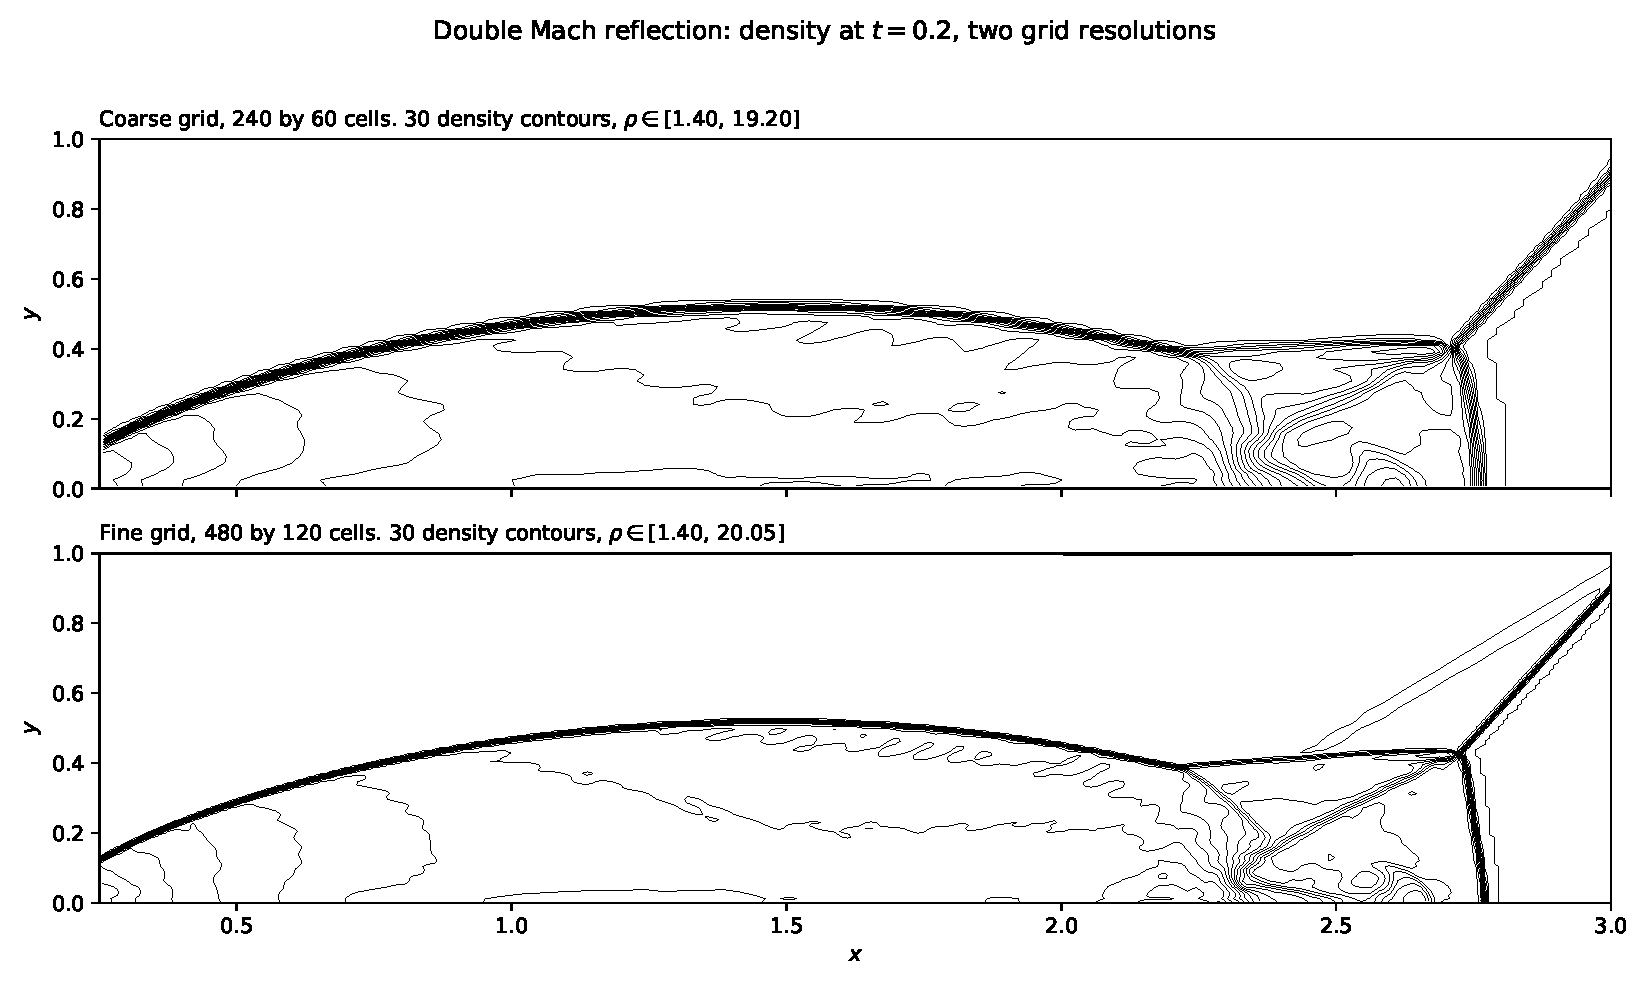
\includegraphics[width=\linewidth]{figures/dmr_density_contours}
\end{center}

\vspace{-4pt}
{\footnotesize The main shock arcs from the lower left. Where it leaves the
wall, a second shock and a jet along the wall form beneath it. The fine grid
holds those features tighter than the coarse grid does.}

\shead{What was verified, in plain words}

\role{Lead Numericist} The incident shock position was compared against the
exact closed-form solution for the shock speed at the same height on both
grids. On the fine grid it agrees to 0.15\,\% of the distance
the shock travelled; on the coarse grid, 0.17\,\%. The
criterion was 1\,\% and it was fixed before the run, not
chosen afterwards.

\role{Lead Researcher} The value of this problem is that it has an exact
answer for one quantity and a hard, sharp, genuinely time-dependent structure
for everything else. Agreeing with the exact part is the necessary condition; it
does not by itself certify the rest of the picture.

\role{Lead Engineer} The benchmark was priced at
20 core-minutes and cost 2.4. The
estimate was the honest one available when it was written and it was high.

\shead{Caveats}

\fcolorbox{boxrule}{boxbg}{\parbox{\dimexpr\linewidth-2\fboxsep-2\fboxrule}{
\textbf{The fine structure behind the main shock is shown here and is not
among the quantities measured.} The second shock and the wall jet beneath the
main front are visible in the picture above. Read them as a picture, not as a
number: no measured value for either is reported on this sheet.\\[2pt]
\textbf{This is an inviscid calculation.} There is no turbulence model in it,
so nothing here says anything about turbulence modelling.\\[2pt]
\textbf{The comparison is against exact theory, not against an experiment.}
No experimental measurement of this configuration exists to compare the rest
of the structure against.
}}

\end{document}
